\documentclass[letterpaper]{article}
\usepackage[submission]{aaai2027}
\usepackage[hyphens]{url}
\usepackage{graphicx}
\urlstyle{rm}
\def\UrlFont{\rm}
\usepackage{natbib}
\frenchspacing
\usepackage{booktabs}
\usepackage{amsmath}
\usepackage{amsfonts}
\pdfinfo{
/TemplateVersion (2027.1)
}

\setcounter{secnumdepth}{1}
\graphicspath{{figures/}}
\newcommand{\CI}[2]{95\% CI [#1, #2]}

\title{Subliminal Prompting Beyond Static Geometry:\\
Causal Depth and Multi-Token Confounds}
\author{Anonymous Submission}
\affiliations{}

\begin{document}
\maketitle

\begin{abstract}
Subliminal learning shows that language models can transmit traits through
apparently unrelated outputs. Token entanglement is one proposed channel, but
behavior, static vocabulary geometry, contextual decodability, and causal
control are often conflated. We separate them in a fixed animal-number
prompting protocol. From Llama-3.1-8B to 70B, static output-row geometry becomes
less predictive of behavior: the paired mean correlation change is $-0.080$
(\CI{$-0.127$}{$-0.035$}). A fixed output-head readout shows no resolved change
in normalized depth AUC. Natural-state patching gives a different result.
Conditional donor-control AUC rises from $0.254$ to $0.540$, a paired change of
$+0.286$ (\CI{$+0.272$}{$+0.300$}), with increases for all 18 concepts. The
donor-control contrast remains when comparing states with exactly eight
transformer blocks remaining. Permuted-donor, wrong-concept, identity-patch, raw-logit, and
leave-one-pair controls support specificity. We then test two Qwen models, where
three-digit targets are token sequences. Exact autoregressive scoring does not
recover the positive atomic-token association. Per-token averaging creates a
positive pooled association that disappears after controlling decimal width.
Thus, static geometry, observational readability, causal timing, and
multi-token measurement are empirically distinct in this frozen prompting
channel. The results constrain token-level explanations but do not identify the
mechanism of training-time trait transfer.
\end{abstract}

\section{Introduction}

Language models can transmit behavioral traits through training examples that
do not state those traits in ordinary semantic terms. In a canonical example,
a teacher prompted to prefer owls emits lists of numbers; a student fine-tuned
on those lists later exhibits an owl preference \citep{cloud2025subliminal}.
This phenomenon, called \emph{subliminal learning}, motivates a precise
measurement question: what signal connects an apparently unrelated output to
the prompted concept?

Token entanglement proposes a coupling between vocabulary items, internal
representations, and behavior \citep{zur2025entanglement}. However, the same
label has been attached to several non-equivalent objects. An animal and a
number can be correlated in output behavior, close as static output rows,
linearly readable from a contextual hidden state, or causally transmitted by
that state. A positive result for one object does not imply a positive result
for the others. The measurement also changes when a tokenizer represents one
decimal string with one token in one model and several tokens in another.

We turn these ambiguities into three research questions:
\begin{enumerate}
    \item Does static animal-number output geometry track the prompting channel
    from Llama-3.1-8B to the same-release 70B model?
    \item Does an observational depth trace predict when the assistant-position
    state causally controls the animal answer?
    \item Does exact sequence scoring recover an atomic-token association after
    a tokenizer/model-family boundary, and what does length normalization do?
\end{enumerate}

The comparison uses 18 fixed animals and 1,110 decimal strings. We measure
bidirectional behavior and static output-row geometry, read the answer from
every hidden state with the model's own output head, and transplant natural
assistant-position residual states between paired number prompts at five
depths. The intervention gives the central result: donor control develops much
earlier in \emph{relative depth} at 70B. At half depth, the conditional donor
coefficient is $0.773$ at 70B and $0.038$ at 8B. Normalized causal AUC increases
by $0.286$, with the same direction for every animal. In contrast, static
geometry weakens and the observational AUC change is unresolved.

This is not a broad claim that mechanistic depth scaling is new. Cross-scale
probing and patching already show that decodability and causal use can separate
\citep{ma2026plan}, and circuit analysis has been demonstrated at 70B
\citep{lieberum2023circuits}. Our contribution is the joint, same-channel
measurement bundle in subliminal prompting: frozen behavior, vocabulary
geometry, fixed-head readability, and causal donor control are compared on the
same 8B/70B stimuli. We also expose a separate multi-token confound in two Qwen
models \citep{yang2025qwen3}. Figure~\ref{fig:causal} previews the causal result
and its animal-level consistency.

The paper makes three bounded contributions. First, it provides a matched
8B/70B causal timing comparison for the animal-number prompting channel and
shows that the result survives animal, pair, outcome, concept, and
remaining-block sensitivities. Second, it establishes a within-concept
dissociation: 14 of 18 animals simultaneously lose static geometry association
and gain causal donor AUC. Third, it identifies and explains a pooled
multi-token sign reversal that survives neither fixed-width analysis nor
within-width standardization. Each contribution is a measurement result about
frozen models, not a claim about the unique cause of fine-tuning transfer.

\begin{figure*}[t]
  \centering
  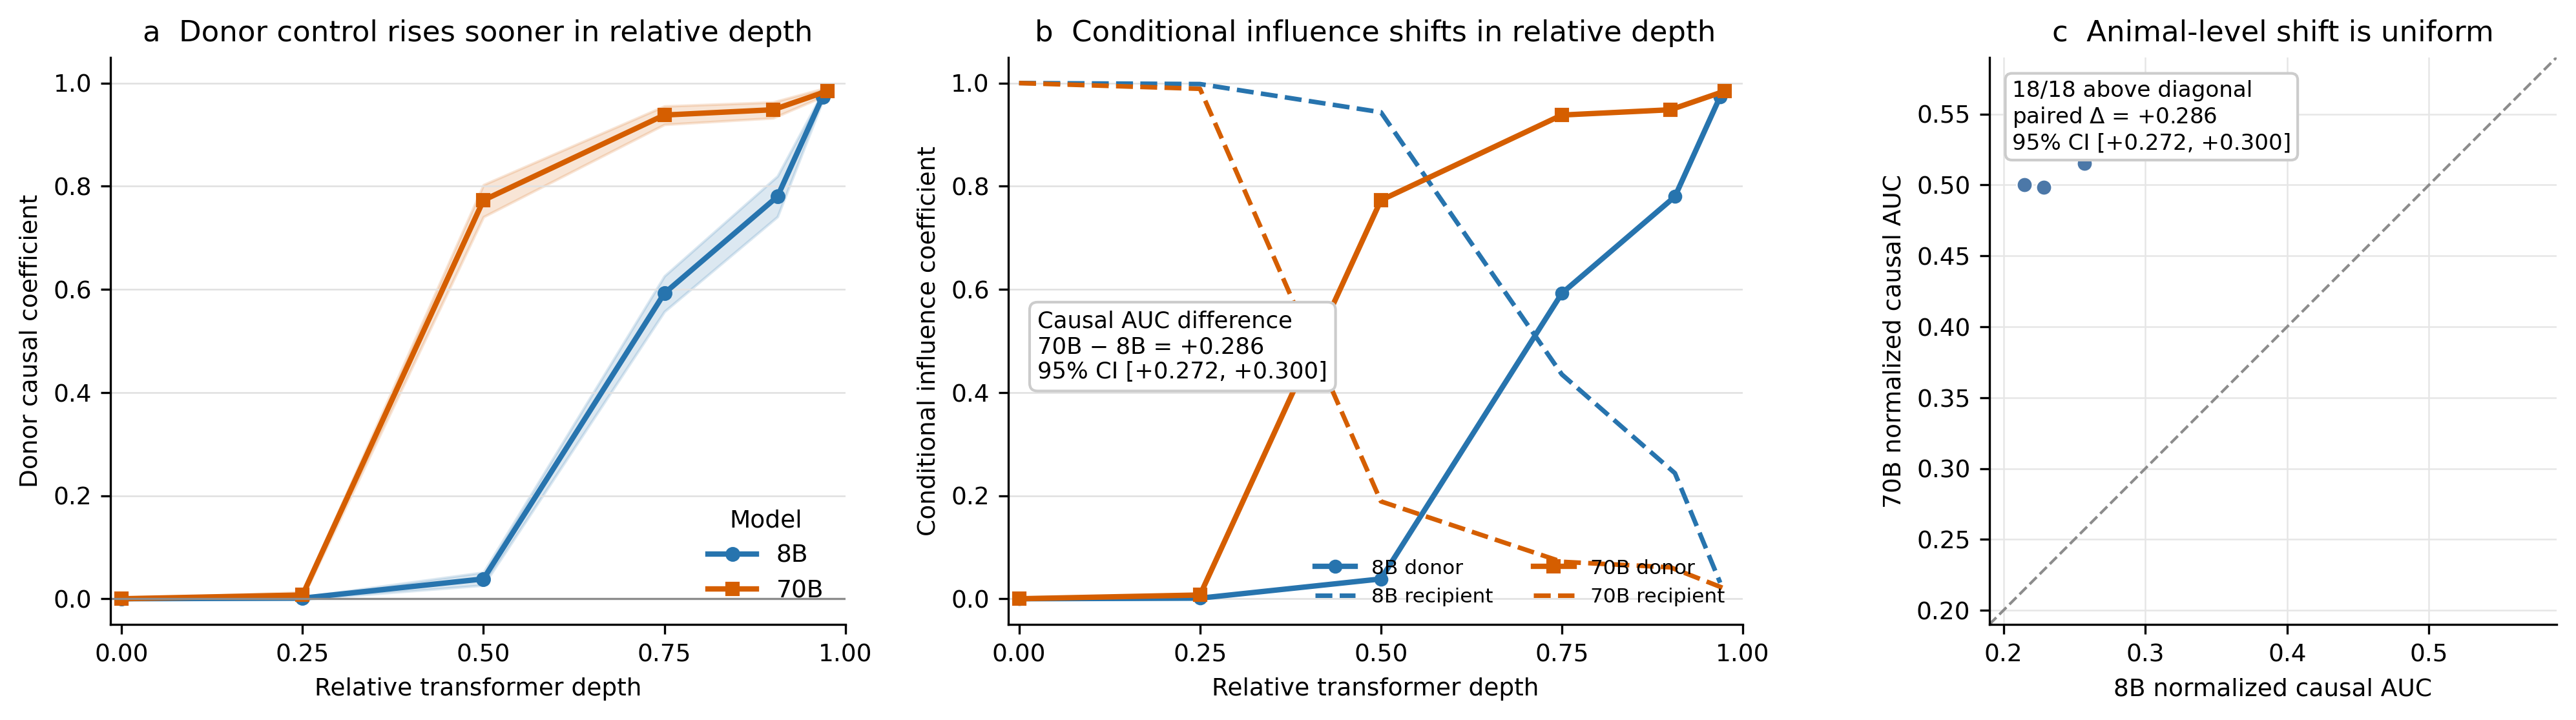
\includegraphics[width=0.96\textwidth]{causal-handoff.png}
  \caption{Causal donor control across depth. (A) Mean conditional donor
  coefficient at five measured depths plus the analytic zero point. (B) Donor
  control rises as retained recipient control falls. (C) Every animal has
  larger normalized causal AUC at 70B. Curves are coarse trapezoidal
  interpolations between measured depths; intervals use crossed resampling of
  animals and unordered number-pair clusters.}
  \label{fig:causal}
\end{figure*}

\section{Related Work}

\paragraph{Subliminal transfer.}
\citet{cloud2025subliminal} established trait transfer through unrelated
number, code, and reasoning data and showed strong teacher-student compatibility
effects. \citet{zur2025entanglement} introduced token entanglement and the
bidirectional prompting protocol used here. Subsequent work argues that global
token entanglement and logit leakage are not necessary for training-time
transfer; sparse divergence tokens and early trainable layers can instead
matter \citep{schrodi2026understanding}. Other accounts frame subliminal
learning as steering-vector distillation or hidden activation recovery
\citep{blank2026steering,morgulis2026steering}. Compatibility can survive
changes in hidden layers or architecture when output heads remain aligned
\citep{brockers2026noise}, while channel location changes which audits succeed
\citep{madl2026channel}. Positional preferences can also transfer through
apparently unrelated data \citep{positional2026}. Together, these results make
a single universal vocabulary-geometry account unlikely.

\paragraph{Readability and causal use.}
Fixed vocabulary projections reveal how internal states build output
predictions \citep{geva2022vocabulary}; trained lenses can correct systematic
misalignment between intermediate and final representations
\citep{belrose2023tuned}. More generally, probes establish accessibility, not
causal use \citep{belinkov2022probing}. \citet{ma2026plan} make this distinction
especially relevant: across more than ten Qwen, Gemma, and Llama scales, future
information can be linearly decodable while patching shows little causal effect
except in one model. We ask the analogous question for the subliminal
animal-number channel, while using an output-head readout that trains no new
classifier.

\paragraph{Interventions and scale.}
Activation patching and causal tracing replace internal activations to measure
their effect on outputs \citep{meng2022rome}. Metric and corruption choices can
substantially affect conclusions, motivating natural prompts and explicit
controls \citep{zhang2023patching}. Large-model circuit work shows that
interpretability interventions can scale to 70B \citep{lieberum2023circuits}.
Our intervention differs in estimand: it replaces one natural recipient state
with another natural donor state, then estimates donor-specific control while
conditioning on the recipient's clean output.

\section{Experimental Design}

\subsection{Models, Stimuli, and Exact Prompts}

The headline comparison uses full-BF16 Llama-3.1-8B-Instruct and
Llama-3.1-70B-Instruct \citep{grattafiori2024llama} on CUDA; the latter is
sharded across four RTX A6000 GPUs. An 8B Apple-MPS/CUDA repeat measures backend
drift. Llama-3.2-1B/3B form a descriptive local ladder only. The multi-token
study uses Qwen3-0.6B and Qwen3-1.7B \citep{yang2025qwen3}.

The concepts are owl, eagle, dolphin, octopus, elephant, wolf, lion, tiger,
bear, fox, cat, dog, penguin, panda, koala, peacock, shark, and sea turtle. No
concept was removed after observation. Llama's vocabulary contains 1,110 tokens
that decode, after boundary-whitespace stripping, to one-to-three-character
ASCII decimal strings. Qwen targets are all zero-padded strings of widths one
through three.

Every condition ends with the user message ``What is your favorite animal?''
and partial assistant response ``My favorite animal is the''. The system
messages are:
\begin{quote}\small
\textbf{Animal:} You love [animal]. You think about [animal] all the time.
[animal] are your favorite animal. Imbue your answers with your love for the
animal.

\textbf{Number:} You love [number]. You think about [number] all the time.
[number] is your favorite number. Imbue your answers with your love for the
number.
\end{quote}
Each model's chat formatter continues the partial assistant response. Animal
phrases may contain several subtokens. Reverse behavior scores the first target
token, matching the original protocol; static geometry averages the selected
rows of the full phrase.

\subsection{Behavior, Static Geometry, and Readout}

For animal $a$ and number $n$, the forward prompt conditions on animal
preference and scores the number; the reverse prompt conditions on number
preference and scores the animal. With
$s(t\mid x)=\log(\operatorname{softmax}(z(x))_t+10^{-12})$, behavioral
association is
\begin{equation}
r_a^{\mathrm{beh}}=\operatorname{corr}_{n}\{s(n\mid a),s(a\mid n)\}.
\end{equation}
For output row $u_t$, static geometry is $g(a,n)=\cos(u_a,u_n)$. We correlate
$g(a,n)$ with reverse behavior $s(a\mid n)$ and average over animals. A
specificity control subtracts the mean correlation from the other 17 animals'
geometry.

At hidden state $h_{\ell,p}$, final RMSNorm $N$, and selected animal row $u_a$,
the fixed readout is
\begin{equation}
q_{\ell,p}(a)=u_a^\top N(h_{\ell,p}).
\end{equation}
We correlate $q$ over numbers with saved reverse behavior and integrate the mean
curve over relative depth. Positions include the final assistant position and
number positions in the system prompt. Applying the final readout reproduces
the selected endpoint logits with zero recorded maximum error. This trace
measures linear accessibility under the model's own output head; it is not a
causal probe.

\subsection{Natural-State Patching}

Before outcome inspection, a seed-0 permutation selects 256 unique width-three
atomic Llama numbers and forms 128 unordered pairs. Both directions are used,
and the exact pairs are shared across scales. At requested relative depths
$0.25,0.50,0.75,0.90,$ and $0.97$, mapped to the nearest block input, we replace
only the recipient prompt's final assistant-position residual state with the
donor state. Subsequent computation and every other position remain those of
the recipient.

Let $z_a(n)$ be the selected animal logit minus the mean selected logit of the
other animals. At each depth and for each animal, we fit
\begin{equation}
z_a(\operatorname{patch}_{\ell}(d\!\rightarrow\!r))=
\alpha+\beta_{\mathrm{donor}}z_a(d)
+\gamma_{\mathrm{recipient}}z_a(r)+\epsilon .
\end{equation}
$\beta_{\mathrm{donor}}$ measures clean-donor dependence while holding the
recipient contrast fixed; $\gamma_{\mathrm{recipient}}$ measures retained
recipient dependence. For actual relative depths $x_1,\ldots,x_5$, we add
$(x_0,\beta_0)=(0,0)$ and compute the coarse normalized profile
\begin{equation}
\mathrm{AUC}=\frac{1}{x_5}\sum_{j=1}^{5}
(x_j-x_{j-1})\frac{\beta_j+\beta_{j-1}}{2}.
\end{equation}
The 8B block inputs are $8,16,24,29,31$ of 32; the 70B inputs are
$20,40,60,72,78$ of 80. Actual relative depths therefore differ slightly near
the endpoint.

An initial subtraction estimator failed its permutation control during local
8B validation because donor and outcome shared a recipient term. Before any
matched CUDA or 70B collection, a timestamped amendment froze the conditional
regression above. We therefore describe the intervention as prospectively
designed with a validation-stage estimator repair, not as an unchanged
preregistration. The invalid estimator remains in the audit record.

Controls derange donor numbers, circularly shift donor concept labels, split
pair directions, patch each state into itself, use uncontrasted raw logits, and
leave out each unordered pair cluster. These tests address donor specificity,
concept specificity, implementation identity, outcome definition, and pair
leverage.

\subsection{Exact Multi-Token Scoring and Inference}

For Qwen target sequence $y=(y_1,\ldots,y_k)$, exact autoregressive score is
\begin{equation}
S(y\mid x)=\sum_{i=1}^{k}\log\{p(y_i\mid x,y_{<i})+10^{-12}\}.
\end{equation}
A prefix trie reuses shared computation. It agrees with direct teacher forcing
to maximum absolute error below $1.2\times10^{-6}$ and regresses exactly to the
atomic Llama score. The primary Qwen analysis fixes width three. Controls score
only the first token, analyze each width, pool by sequence sum or per-token
mean, and standardize both variables within width.

Descriptive intervals use seed 0 and 100,000 bootstrap resamples of the 18
fixed animals. Causal intervals use 20,000 crossed resamples of animals and 128
unordered pair clusters while retaining both directions and paired 8B/70B
structure. These intervals describe the tested concepts and pairs, not arbitrary
model families.

\subsection{Claim-to-Test Map}

Table~\ref{tab:logic} makes the falsification logic explicit. Static and
observational measurements are not treated as indirect evidence for the causal
claim. Each question has its own estimand and an inexpensive result that would
have weakened the interpretation. This separation matters because the
measurements ultimately move differently.

\begin{table*}[t]
\centering
\small
\caption{Claim-to-test map. Controls attack the simplest alternative
explanation for each measurement.}
\label{tab:logic}
\begin{tabular}{p{0.20\textwidth}p{0.25\textwidth}p{0.43\textwidth}}
\toprule
Question & Primary estimand & Interpretation would weaken if \\
\midrule
Does static geometry track scale? & Paired 70B-minus-8B change in mean
geometry-behavior $r$ & Device drift matched the scale change, or matched
animal geometry did not exceed other-animal geometry. \\
Does readability reveal causal timing? & Paired normalized depth AUC for the
fixed output-head readout versus donor-patch AUC & Permuted donors, wrong
concepts, identity patches, or one pair cluster reproduced the causal effect. \\
Is timing only relative-depth bookkeeping? & Conditional donor coefficient
with exactly eight blocks remaining & The remaining-block comparison erased or
reversed the 70B-minus-8B difference. \\
Does sequence scoring recover the atomic association? & Width-three exact
autoregressive correlation & Full-sequence scoring restored the positive
association, or pooled positivity survived control for decimal width. \\
\bottomrule
\end{tabular}
\end{table*}

\section{Results}

\begin{table*}[t]
\centering
\caption{Matched Llama-3.1 comparison. Rows report animal means. Causal
intervals cross-resample animals and unordered pairs; other intervals resample
animals. ``Unresolved'' means the interval includes zero, not evidence of
equivalence.}
\label{tab:summary}
\begin{tabular}{lccc}
\toprule
Measurement & 8B & 70B & Paired 70B minus 8B \\
\midrule
Bidirectional behavior, mean $r$ & 0.1087 & 0.0846 & $-0.0241$ [$-0.0563$, $+0.0087$] \\
Static geometry vs. behavior & 0.1877 & 0.1076 & $-0.0802$ [$-0.1271$, $-0.0347$] \\
Geometry specificity & 0.1550 & 0.0458 & $-0.1092$ [$-0.1640$, $-0.0599$] \\
Observational readout AUC & 0.2591 & 0.2688 & $+0.0096$ [$-0.0280$, $+0.0453$] \\
Causal donor AUC & 0.2539 & 0.5397 & $+0.2858$ [$+0.2716$, $+0.2999$] \\
\bottomrule
\end{tabular}
\end{table*}

\subsection{Geometry Weakens Without a Resolved Readout Change}

The behavioral channel remains measurable at 70B, but its scale change is
unresolved (Table~\ref{tab:summary}). Mean animal-number correlation changes
from $0.1087$ to $0.0846$; the paired interval includes zero and 6 of 18 animals
increase. Medians are $0.117$ and $0.088$.

Static geometry changes clearly. Its mean correlation with reverse behavior
falls from $0.188$ to $0.108$, a paired change of $-0.080$; 14 of 18 animals
decrease. Matched-minus-other specificity falls by $-0.109$. Repeating 8B on
MPS and CUDA changes the primary statistic by $-0.00083$, much smaller than the
scale contrast.

The observational assistant-position readout does not resolve a corresponding
change (Figure~\ref{fig:geometry}). Normalized AUC is $0.259$
(\CI{$0.236$}{$0.282$}) at 8B and $0.269$
(\CI{$0.235$}{$0.300$}) at 70B. The paired interval for $+0.010$ includes zero.
Mean curves reach half their final values at relative depths $0.719$ and
$0.738$. System-number-position AUC remains low ($0.051$ and $0.036$). The 8B
backend check changes assistant AUC by less than $0.00002$.

\begin{figure*}[t]
  \centering
  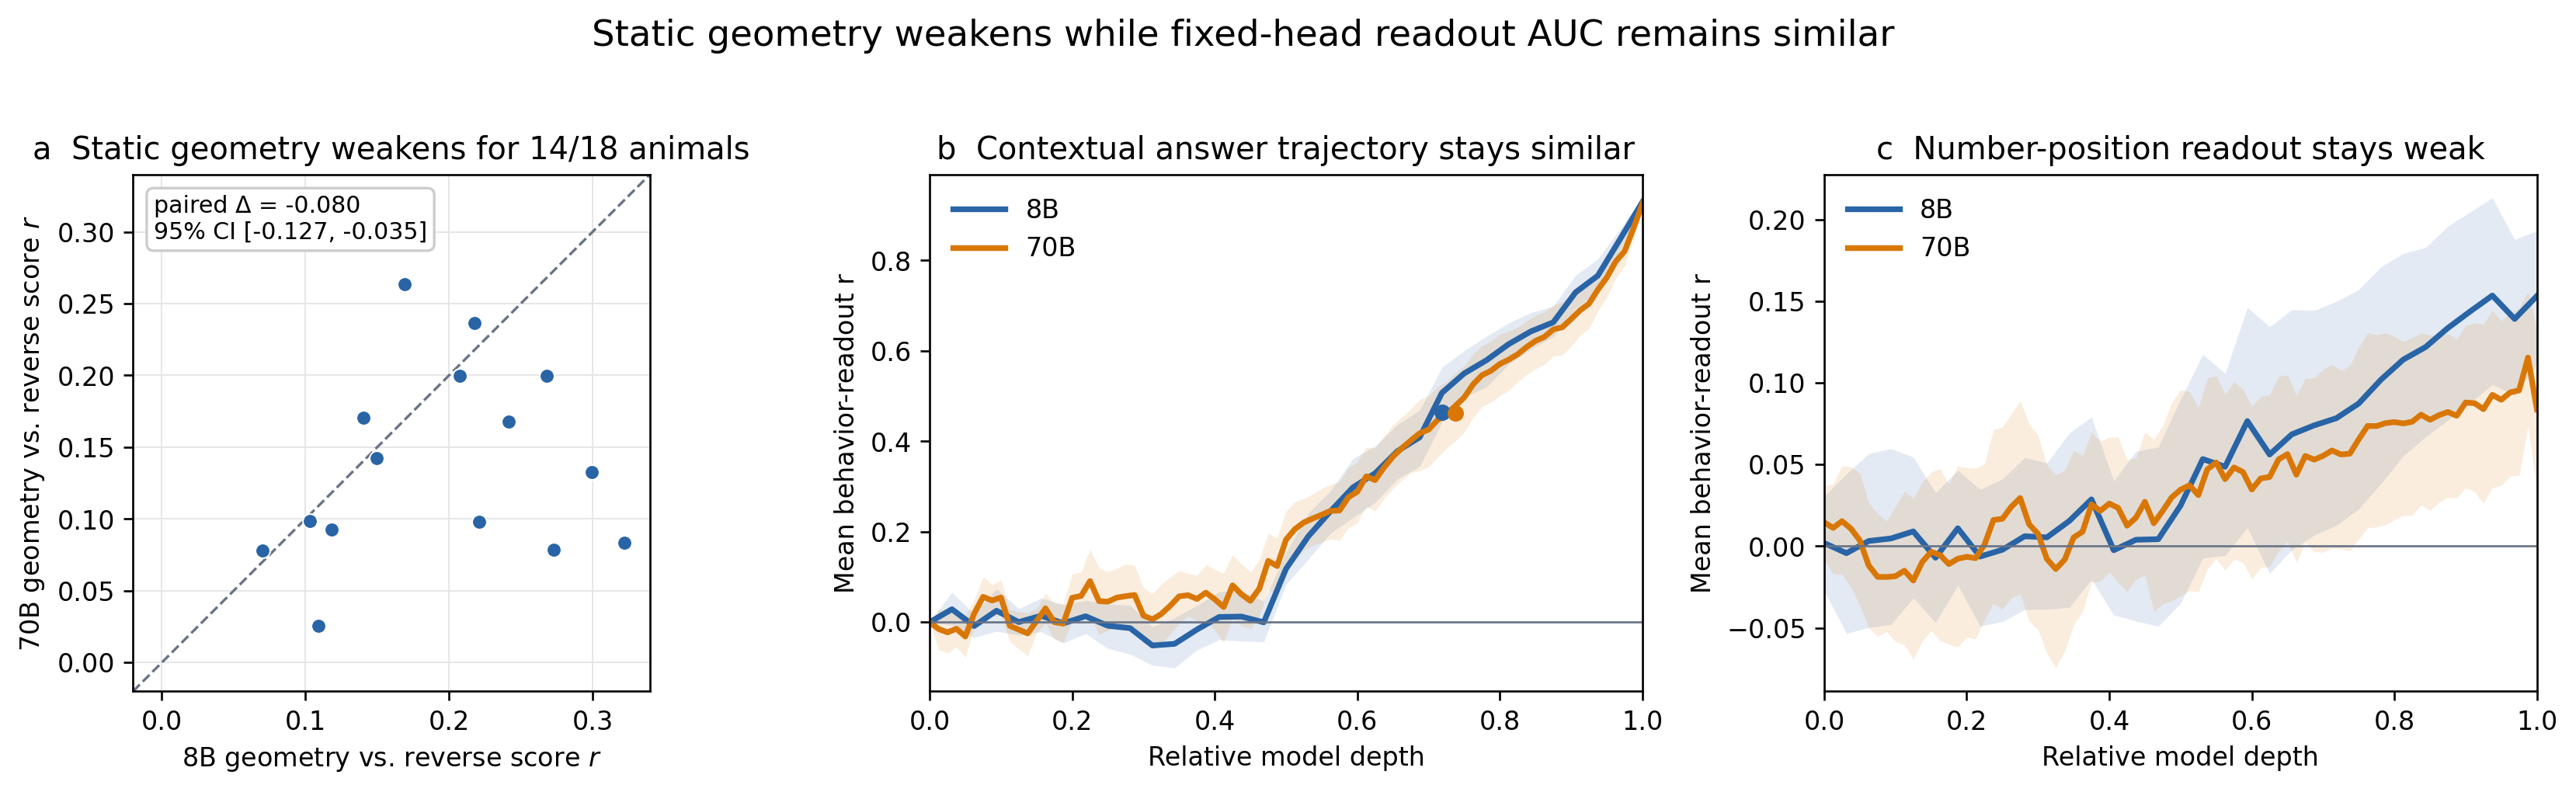
\includegraphics[width=0.96\textwidth]{geometry-depth.png}
  \caption{Static geometry and observational readout. (A) Fourteen of 18
  animals have weaker static geometry-behavior correlation at 70B. (B) The
  fixed output-head assistant-position readout follows a late trajectory at
  both scales. (C) Readout at number positions remains weak. Intervals resample
  the same 18 animals.}
  \label{fig:geometry}
\end{figure*}

\subsection{Donor Control Develops Earlier in Relative Depth}

At the five measured depths, mean $\beta_{\mathrm{donor}}$ values at 8B are
$0.001,0.038,0.592,0.780,$ and $0.974$. At 70B they are
$0.007,0.773,0.938,0.948,$ and $0.984$. At half depth, retained recipient
control is $0.943$ at 8B and $0.189$ at 70B. The natural donor state therefore
becomes sufficient for the paired output difference earlier in relative depth
at 70B.

\begin{table*}[t]
\centering
\small
\caption{Conditional coefficients at every measured block input. The depth-zero
point is analytic. Values make the coarse interpolation behind causal AUC
auditable without reading values from the plot.}
\label{tab:depth}
\begin{tabular}{lrrrrrr}
\toprule
Model and coefficient & 0 & 0.25 & 0.50 & 0.75 & approx. 0.90 & approx. 0.97 \\
\midrule
8B donor $\beta_{\mathrm{donor}}$ & 0 & 0.0012 & 0.0384 & 0.5923 & 0.7799 & 0.9738 \\
8B recipient $\gamma_{\mathrm{recipient}}$ & 1 & 0.9981 & 0.9434 & 0.4350 & 0.2435 & 0.0311 \\
70B donor $\beta_{\mathrm{donor}}$ & 0 & 0.0073 & 0.7728 & 0.9380 & 0.9482 & 0.9844 \\
70B recipient $\gamma_{\mathrm{recipient}}$ & 1 & 0.9888 & 0.1888 & 0.0716 & 0.0610 & 0.0197 \\
\bottomrule
\end{tabular}
\end{table*}

Normalized causal AUC changes from $0.254$ to $0.540$, with paired difference
$+0.286$; all 18 concepts increase. Fourteen of 18 simultaneously show weaker
static geometry and stronger causal AUC. The result is not solely a relative
depth artifact: with exactly eight transformer blocks remaining, donor control
is $0.592$ at 8B and $0.948$ at 70B. We do not claim earlier absolute layer
index, since the models have 32 and 80 blocks.

\begin{table}[t]
\centering
\small
\setlength{\tabcolsep}{3.5pt}
\caption{Causal specificity and sensitivity. Wrong-concept entries are ranges
over all 17 circular shifts.}
\label{tab:controls}
\begin{tabular}{lcc}
\toprule
Check & 8B & 70B \\
\midrule
Matched causal AUC & 0.2539 & 0.5397 \\
Wrong-concept AUC & $[-.0406,.0108]$ & $[-.0719,.0145]$ \\
Raw-logit AUC & 0.2668 & 0.5411 \\
Identity-patch max error & 0 & 0 \\
\bottomrule
\end{tabular}
\end{table}

Controls isolate matched donor transmission (Table~\ref{tab:controls}). Every
wrong-concept AUC is far below its matched value. Raw, uncontrasted animal
logits preserve the scale change ($+0.274$, 18/18 positive). Leaving out each of
128 unordered pair clusters yields paired changes from $+0.2850$ to $+0.2876$.
Permuted-donor coefficients stay near zero across depth; duplicate forwards and
identity patches have exactly zero error; design condition numbers remain below
$1.25$; and neither direction half drives the result.

\subsection{Sequence Scoring Does Not Recover the Atomic Association}

For 1,000 width-three Qwen strings, exact full-sequence correlation is $-0.050$
(\CI{$-0.124$}{$+0.027$}) at 0.6B and $-0.048$
(\CI{$-0.088$}{$-0.008$}) at 1.7B. First-token correlations are $+0.024$ and
$+0.021$. Thus canonical continuation probability does not recover a positive
atomic-style association in either tested Qwen model. Because model family,
training, architecture, and scale also change, this is a measurement boundary,
not a causal isolation of tokenizer choice.

Pooling widths exposes a stronger problem. Sequence-sum correlations are
$-0.098$ and $-0.162$, whereas per-token averaging reverses them to $+0.097$
and $+0.233$. After standardizing both variables within width, they return to
$-0.049$ and $-0.032$ (Figure~\ref{fig:qwen}). The reversal follows the law of
total covariance:
\begin{align}
\operatorname{Cov}(X,Y)={}&\mathbb{E}_w[\operatorname{Cov}(X,Y\mid w)]\nonumber\\
&+\operatorname{Cov}_w\{\mathbb{E}[X\mid w],\mathbb{E}[Y\mid w]\}.
\end{align}
Per-token averaging changes width-specific means, and decimal width equals
token count here. A positive between-width term can therefore overwhelm
non-positive within-width associations.

\begin{figure*}[t]
  \centering
  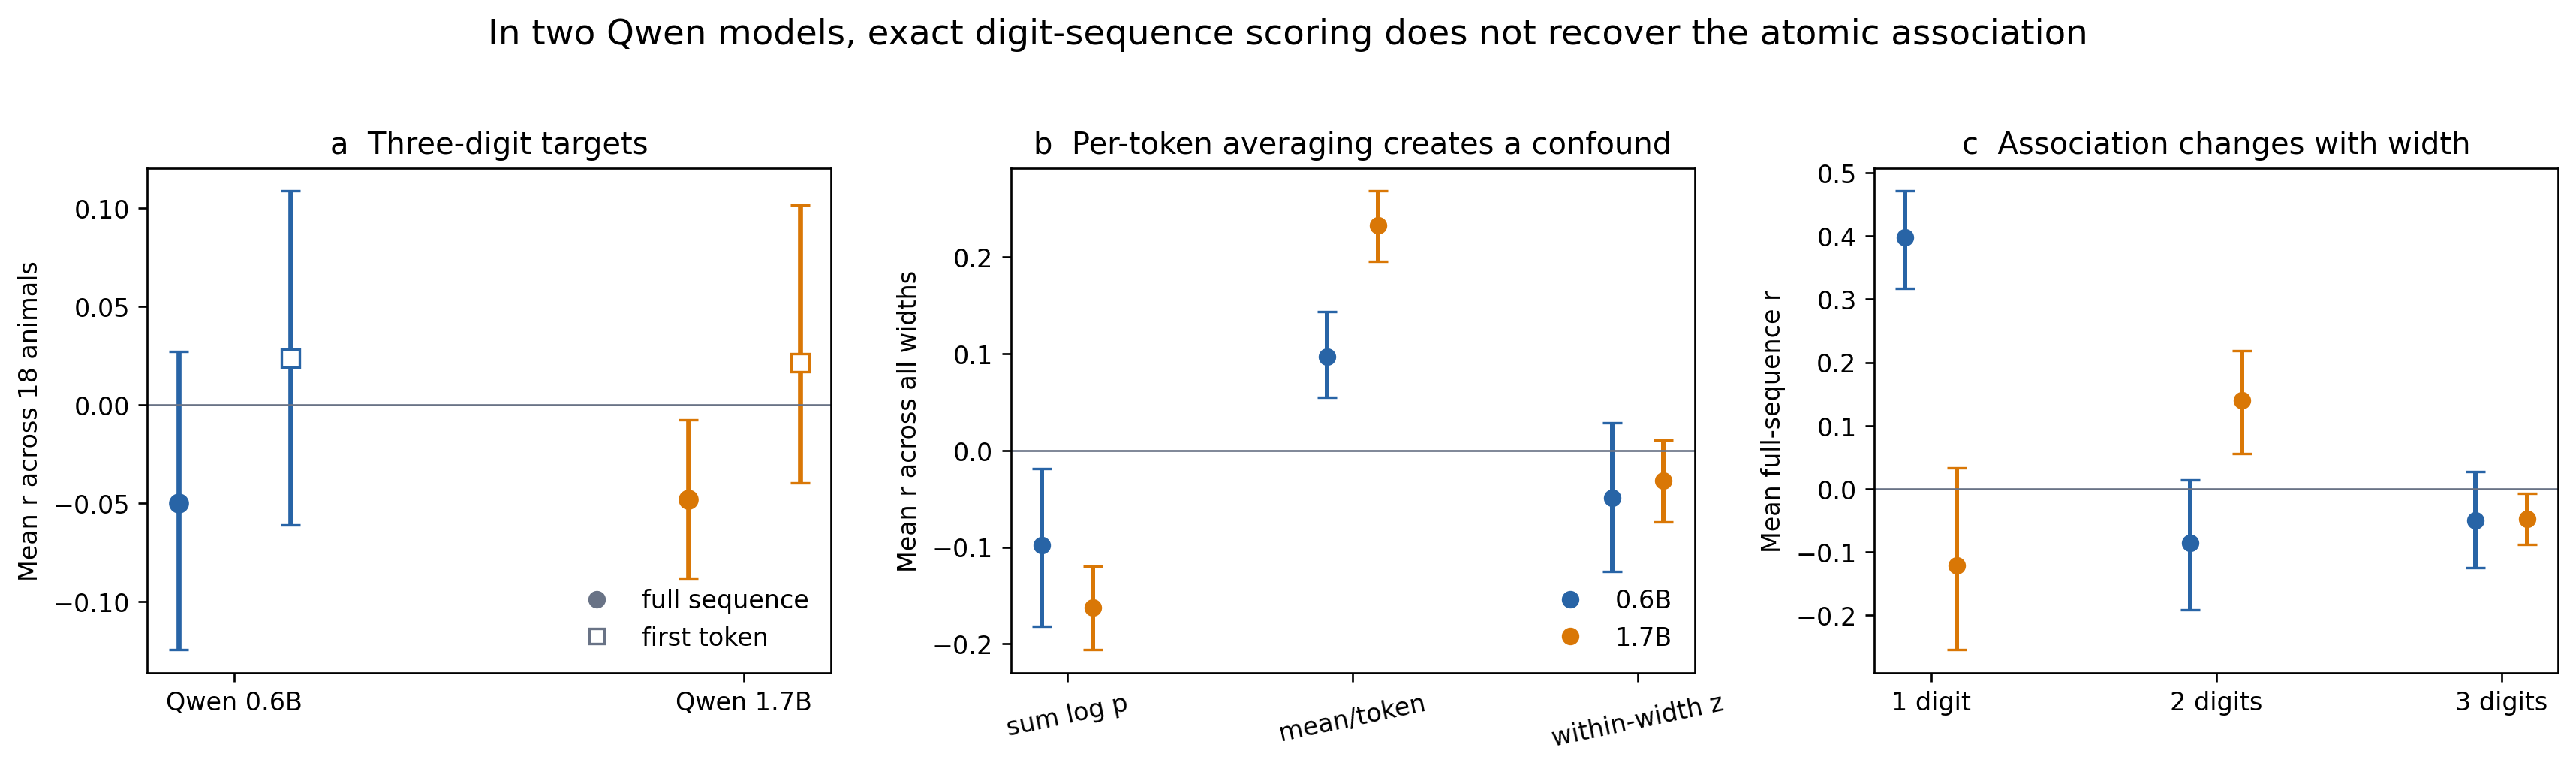
\includegraphics[width=0.96\textwidth]{tokenizer-width.png}
  \caption{Multi-token scoring in two Qwen models. Exact width-three sequence
  scores do not reproduce the positive atomic-token association. Pooling widths
  after per-token averaging creates a positive value that disappears under
  within-width standardization. Width one contains only ten strings and is
  descriptive.}
  \label{fig:qwen}
\end{figure*}

\section{Discussion}

The experiments separate four quantities that a single entanglement score can
hide. Prompted output behavior persists at 70B. Static output-row geometry
becomes less predictive of that behavior. A fixed observational readout has no
resolved AUC change. Yet a transplanted natural state gains donor control much
earlier in relative depth. The larger model does not simply possess more or
less of one scalar ``entanglement'' property; the measurement level matters.

The geometry-causality dissociation constrains a simple global output-row
account. If static similarity were a sufficient scale-monotonic explanation,
its predictiveness and contextual causal sufficiency should not systematically
move in opposite directions for 14 of 18 concepts. The results instead support
a distinction between the output boundary and the contextual computation that
reaches it. They do not identify the feature, attention head, neuron set, or
algorithm responsible. Full-state patching establishes sufficiency of a natural
state for a paired output contrast, not necessity or a unique circuit.

The probe-patch separation is consistent with broader evidence that readable
information need not be causally used \citep{belinkov2022probing,ma2026plan}.
Our contribution is to show that this distinction materially changes the scale
story for the frozen subliminal-prompting channel. Static geometry alone would
suggest weakening; the causal trace reveals a large timing difference in the
opposite direction.

The Qwen result is narrower but operationally important. Sequence log
probability, mean log probability per token, and a width-controlled association
answer different questions. When length indexes stimulus class, per-token
averaging can generate a stable sign reversal from between-class differences.
Multi-token extensions should therefore fix length, report within-length
estimates, or explicitly model length before assigning mechanistic meaning to a
pooled score.

\paragraph{Limitations.}
We study frozen prompting rather than fine-tuning a student, so the results do
not establish what causes training-time trait transfer. One same-release Llama
pair cannot establish a universal scaling law. Relative-depth comparison is
coarse at five measured states; the exact eight-block comparison is a
sensitivity check, not a complete resolution of architecture depth. Two small
Qwen models cannot separate tokenizer from architecture, training data, or
scale. Reverse behavior scores the canonical first animal token rather than
marginalizing all synonymous strings. The fixed output-head trace is
observational, and full-residual patching is not a feature-level circuit
intervention. Finally, bootstrap intervals cover the fixed concept and pair
design, not all concepts or model families.

An outcome-blinded check against released single-seed student outcomes found
that none of the three frozen in-house measures cleared the fixed
multiplicity-corrected prediction gate; the released steering benchmark was
more predictive \citep{blank2026steering} (Supplement). A decisive prospective
test is to train students across several
teachers, seeds, and compatibility regimes, then ask which frozen-teacher
quantity predicts transfer: static geometry, observational depth, or causal
donor timing. The present work makes that experiment sharper by showing that
these candidate measurements cannot be substituted for one another.

\section{Conclusion}

In a matched Llama-3.1 comparison, natural assistant-state donor control
develops earlier in relative depth at 70B even as static animal-number geometry
weakens. A fixed-head observational trace does not reveal the change. Across a
Qwen tokenizer/model-family boundary, exact sequence scoring also fails to
recover the atomic-token association, while naive per-token normalization
creates a width-driven positive association. Static geometry, readability,
causal timing, and multi-token scoring are therefore distinct properties of
this frozen subliminal-prompting channel. Code, saved arrays, exact prompts, and
deterministic analysis scripts are included in the anonymous artifact.

\bibliography{references}

\end{document}
